\documentclass[12pt]{article}
\usepackage[margin=1in]{geometry}

% Start of preamble
%==========================================================================================%
% Required to support mathematical unicode
\usepackage[warnunknown, fasterrors, mathletters]{ucs}
\usepackage[utf8x]{inputenc}

% Always typeset math in display style
%\everymath{\displaystyle}

% GROUPOIDS FONT!
\usepackage{eulervm}
\usepackage{charter}

% Standard mathematical typesetting packages
\usepackage{amsthm, amsmath, amssymb}
\usepackage{mathtools}  % Extension to amsmath

% Symbol and utility packages
\usepackage{cancel, textcomp}
\usepackage[mathscr]{euscript}
\usepackage[nointegrals]{wasysym}

% Extras
\usepackage{physics}  % Lots of useful shortcuts and macros
\usepackage{tikz-cd}  % For drawing commutative diagrams easily
\usepackage{color}  % Add some color to life
\usepackage{microtype}  % Minature font tweaks
%\usepackage{pgfplots} % plots

\usepackage{enumitem}
\usepackage{titling}

\usepackage{graphicx}

% Common shortcuts
\def\mbb#1{\mathbb{#1}}
\def\mfk#1{\mathfrak{#1}}

\def\bN{\mbb{N}}
\def\bC{\mbb{C}}
\def\bR{\mbb{R}}
\def\bQ{\mbb{Q}}
\def\bZ{\mbb{Z}}

% Sometimes helpful macros
\newcommand{\floor}[1]{\left\lfloor#1\right\rfloor}
\newcommand{\ceil}[1]{\left\lceil#1\right\rceil}
\DeclarePairedDelimiterX\set[1]\lbrace\rbrace{\def\given{\;\delimsize\vert\;}#1}

% Some standard theorem definitions
\newtheorem{theorem}{Theorem}[section]
\newtheorem{corollary}{Corollary}[theorem]
\newtheorem{lemma}[theorem]{Lemma}

\theoremstyle{definition}
\newtheorem{definition}{Definition}[section]

\theoremstyle{remark}
\newtheorem*{remark}{Remark}

% End of preamble
%==========================================================================================%

% Start of commands specific to this file
%==========================================================================================%

\newcommand{\R}{\mathbb{R}}
\renewcommand{\ip}[2]{\langle #1, #2 \rangle}
\newcommand{\mg}[1]{\| #1 \|}
\newcommand{\linf}[1]{\max_{1\leq i \leq #1}}
\newcommand{\ve}{\varepsilon}
\renewcommand{\qed}{\hfill\qedsymbol}
\newcommand{\seq}[2]{\qty(#1_#2)_{#2=1}^{\infty}}
%\renewcommand{\geq}{\geqslant}
%\renewcommand{\leq}{\leqslant}


%==========================================================================================%
% End of commands specific to this file

\title{Insert Title}
\date{\today}
\author{Rohan Mukherjee}

\begin{document}
	\maketitle
	\begin{enumerate}[leftmargin=\labelsep]
		\item The counterexample for this question is going to be $f(x) \equiv c$, where $c \in \R$. Clearly $f' = 0$ for all $x \in [0, 1]$, and there are certainly infinitely many points in $[0, 1]$.
		
		\item 
		\begin{enumerate}
			\item The counterexample is 
			\begin{align*}
				f(x)=
				\begin{cases}
					\exp(-\frac 1x)\sin(\frac 1x) \quad x > 0 \\
					0, \quad x \leq 0
				\end{cases}
			\end{align*}
			Note that outside of zero, this function is the product/composition of two infinitely differentiable functions, and is therefore itself infinitely differentiable (who's derivative is always given by the chain rule). It suffices to show the derivatives always exist at the origin. First, I show that the function is continuous at the origin. $\lim_{x \to 0^+} f(x) = \lim_{x \to \infty} e^{-x}\sin(x) = 0$. Now I claim that the derivative at the origin is continuously 0.
		
			\begin{lemma}
				All derivatives of the above $f(x)$ are of the form \begin{align}
					e^{-1/x} \sum_k P_k\qty(\frac1x)\sin / \cos (\frac 1x)
				\end{align}, where $P_k\qty(\frac 1x)$ is a polynomial with only positive powers in $\frac 1x$, and the sum is finite.
			\end{lemma}
		
			\begin{proof}
				The base case is clear: $f'(x) = e^{-1/x}\cos(\frac 1x) \cdot -\frac 1{x^2} -\frac 1{x^2} e^{-1/x}\sin(\frac 1x)$
				
				Note first that $\dv{x} x^{-n} = -nx^{-n-1}$ when $n \in \bN$, and as a polynomial in $x^{-1}$ is simply a finite sum of those terms, it's derivative is of course another polynomial in $x^{-1}$. The derivative of $\sin(\frac 1x) = -\frac1{x^2}\cos(\frac 1x)$, $\dv{x} \cos(\frac1x) = \frac1{x^2}\sin(\frac1x)$, so in any case the derivatives of the terms inside the sum will be a polynomial in $x^{-1}$ multiplied by either $\sin$ or $\cos$, given by the product rule. Finally, the derivative of $e^{-1/x}$ is $-\frac1{x^2}e^{-1/x}$, so bringing the $-\frac1{x^2}$ inside the sum will make the function's derivative of the above form. Finally, the product rule was applied a finite number of times, to a finite number of terms, so of course the sum is finite.
			\end{proof}
		
			What is commonly known is that $x^n/e^x \to 0$ for every positive $n$ as $x \to \infty$. Take any function of the form in (1). Bring the $e^{-1/x}$ term in, and it suffices to show that each term in the sum goes to 0. Now, $|e^{-1/x}P(x^{-1})\sin/\cos(x^{-1})| \leq |e^{-1/x}P(x^{-1})|$. Now applying the substitution $u = x^{-1}$, and using the fact stated above, shows that this limit goes to 0. A sum of a lot of 0s is of course another 0, so we are done.
			\item We use the same trick as last time. Consider the function: \begin{align*}
				g(x) = \begin{cases}
					-e^{-1/x}\psi(1/x), \quad x > 0 \\
					0, \quad x \leq 0
				\end{cases}
			\end{align*}. As one can see from the definition of $\psi(x)$, this function is going to have infinitely many local minima, and zero local maxima, contradicting the claim.
			\item If you look to the bump function in question 2, on the interval $[0, 11]$ it has 10 strict local maxima and 0 strict local minima. This could also work for $[0, 1]$ as we could simply send $x \to 10x$ to "squish" our function to the right interval, which disproves the claim.
		\end{enumerate}
	
	\item 
	We construct a counterexample. Consider the "bump" function:
	\begin{align*}
		\psi(x) = \exp(-\frac1{1-(4(x-1/2))^2})
	\end{align*} for $\frac14 \leq x \leq \frac34$, and $0$ on $[0, \frac14] \cup [\frac34, 1]$. Here is a picture:
	
	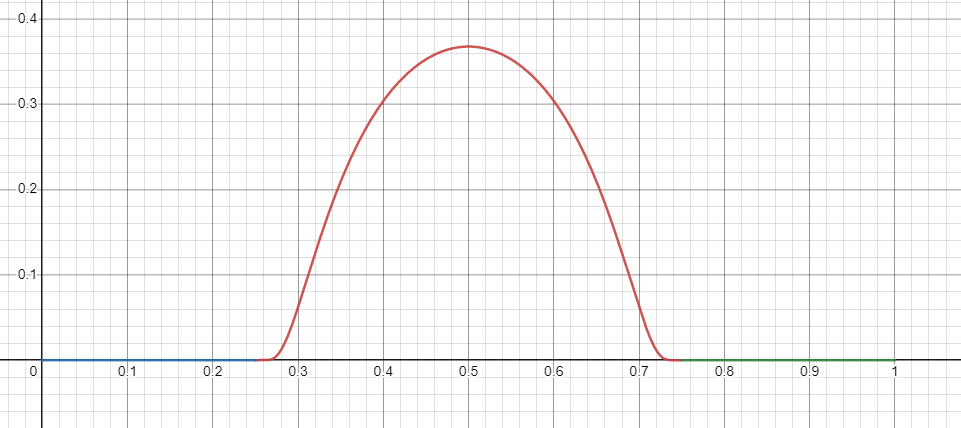
\includegraphics[scale=0.5]{function.png}
	
	This function can clearly be extended to a 1-periodic function (simply shift this right/left by 1), with the peaks 1 apart from each other. Also, there is 1 and only 1 strict local extrema, at the peak. This contradicts the claim as 1 is not even. This bump function is known to be infinitely differentiable, from the wikipedia page on the topic (or one could see this as it is a composition of two infinitely differentiable, things, and at the points where it couldn't be infinitely differentiable, the $e^x$ term dominates).
	
	\item
	\begin{enumerate}
		\item $\pdv{f}{x} = 3x^2-y^2-2x, \pdv{f}{y} = -2yx+y^2$. We see that the set of solutions to $\grad{f} = 0$ is $\set{(0, 0), (2/3, 0), (-2, -4)}$. The hessian of $f$ is 
		\begin{align*}
			\begin{pmatrix}
				6x-2 && 2y \\
				2y && -2x+2y
			\end{pmatrix}
		\end{align*}
		Therefore the origin is a degenerate critical point. For the point $(2/3, 0)$, the determinant of the hessian is negative, so $f$ has a saddle point there. The point $(-2, -4)$ has positive determinant, and $f_{xx}(-2, -4) < 0$, so $f$ has a local maximum there. Along the line $r(t) = (0, t)$, $f(r(t))=t^2,$ which clearly has a local minimum at the origin. Along the line $r(t) = (t, 0)$, $f(r(t)) = (t-1) \cdot t^2$, which has a local maximum at the origin. So the origin is a saddle point.
		
		\item 
		Finding the gradient and setting it to the zero vector, we get the points $\set{(\pm 1, 0), (0, \pm 1), (0, 0)}$. Plugging these into the determinant of the hessian, which is: $(-32x^6-64x^4y^2+96x^4-40x^2y^4+104x^2y^2-56x^2-8y^6+36y^4-44y^2+8)e^{-2x^2-2y^2}$, we see that $(0, \pm 1)$ are saddle points, as they make the hessian determinant negative. The rest have positive determinant, and checking with $f_{xx}$ we get that $(0, 0)$ gives a local minima, and $(\pm 1, 0)$ give local maxima.
		
		\item 
		The function is "symmetric" in the variables $x, y, z$ (meaning you could apply $x \to y, y \to z, z \to x$ or any other permutation and you would get the same function), so it suffices to only look at 3 solutions to the gradient: $(0, 0, z), (0, y, 4-y), (1, 1, 1)$. AM-GM shows that (1, 1, 1) is the maximum value among all positive $x, y, z$, so it must therefore be a local maximum (as $xyz$ is maximized by having them all be equal, and $x+y+z$ is minimized by them all being equal). The other two classes of solutions are all degenerate. First note that you could get all the other solutions by doing any of the 6 permutations described briefly above. In the $(0, 0, z)$ case, the function is constantly zero--and therefore has neither a local min/max/saddle point. The same scenario plays out with $(0, y, 4-y)$.
	\end{enumerate}
	\item 
	We see that $f(x, y) = y^2-3x^2y+2x^4$, so
	\begin{align*}
		\grad{f} = 
		\begin{pmatrix}
			-6xy+8x^3 \\
			2y-3x^2
		\end{pmatrix}
	\end{align*}
	Clearly now the origin is a critical point, and we see that the hessian of $f$ is:
	\begin{align*}
		\begin{pmatrix}
			-6y+24x^2 && -6x \\
			-6x && 2
		\end{pmatrix}
	\end{align*}
	At the origin this matrix will have its top row all 0s, so it has det 0, i.e. the origin is a degenerate critical point. Any line through the origin is of the form $r(t) = (at, bt)$, where $a, b \in \R$. Then $g(t) = f(r(t)) = b^2t^2 - 3a^2bt^3 + 2a^4t^4$. We see that $g'(t) = 2b^2t - 9a^2bt^2+8a^4t^3$, where clearly $t = 0$ which corresponds to the origin makes this $0$. Taking another derivative, we see that $g''(t) = 2b^2+tP(t)$, where $P(t)$ is a polynomial in $t$ of degree $>1$. Then $g''(0) = 2b^2$, which is strictly greater than 0, unless $b=0$. If $b=0$, then $g(t) = 2a^4t^4$, which clearly has a local minimum at $t=0$ for all non-zero values of $a$ (note if $a=0$ then we don't have a line). As all linear paths have a local min at the origin, we see that we must use a nonlinear curve. Although most curves also have a local min at the origin, I found one that works: $(x,y)=(x,\frac32x^2)$. This function has a local maximum at the origin, so the origin is in fact a saddle point.
	\end{enumerate}
\end{document}